
\section{Solution}
\label{sec:auswertung}

\begin{itemize}
    \item[a)]
        As the first part of the exercise was to just implement the constructor we don't have anything to show for this part besides the code.
    \item[b)]
        In exercise part b we were supposed to write a measurment and equilibrate function that simulated the interaction between particles.
        Three different simulations were asked for.
        One with 16 particles, one with 64 and one with 256.
        After the system were in a rough equilibrium we measured the kinetic and potential energy of the system as well as the temperature.
        The resulting plots can be seen below.
        \FloatBarrier
        \begin{figure}
            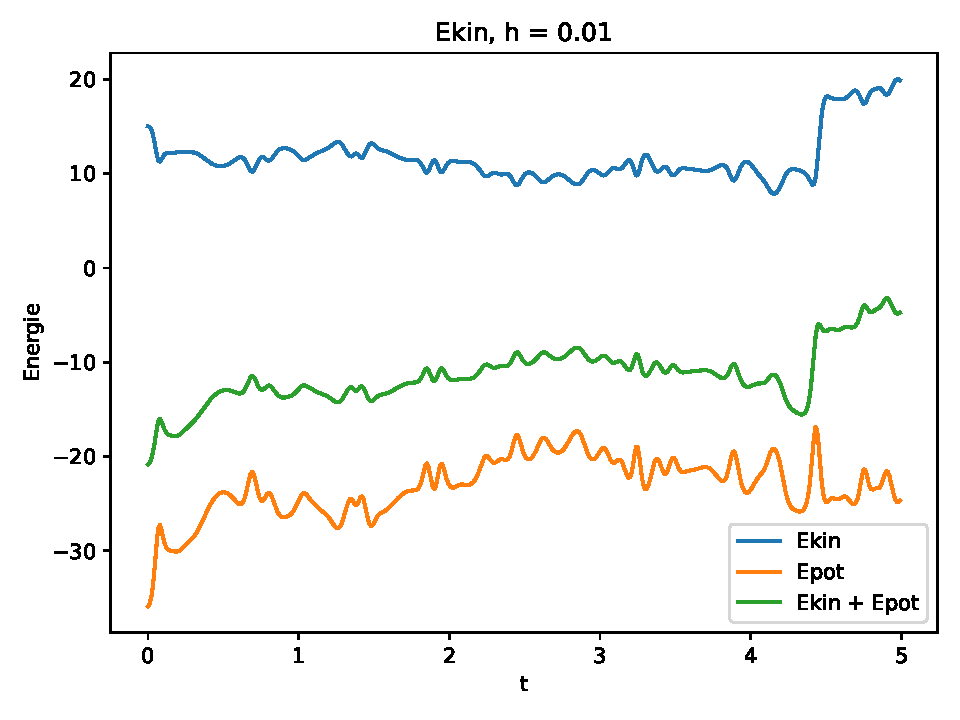
\includegraphics[width=\textwidth]{images/plot_E_16.pdf}
            \caption{The energy of the 16 particle simulation over 5 seconds with a stepsize of 0.001.}
        \end{figure}
        \begin{figure}
            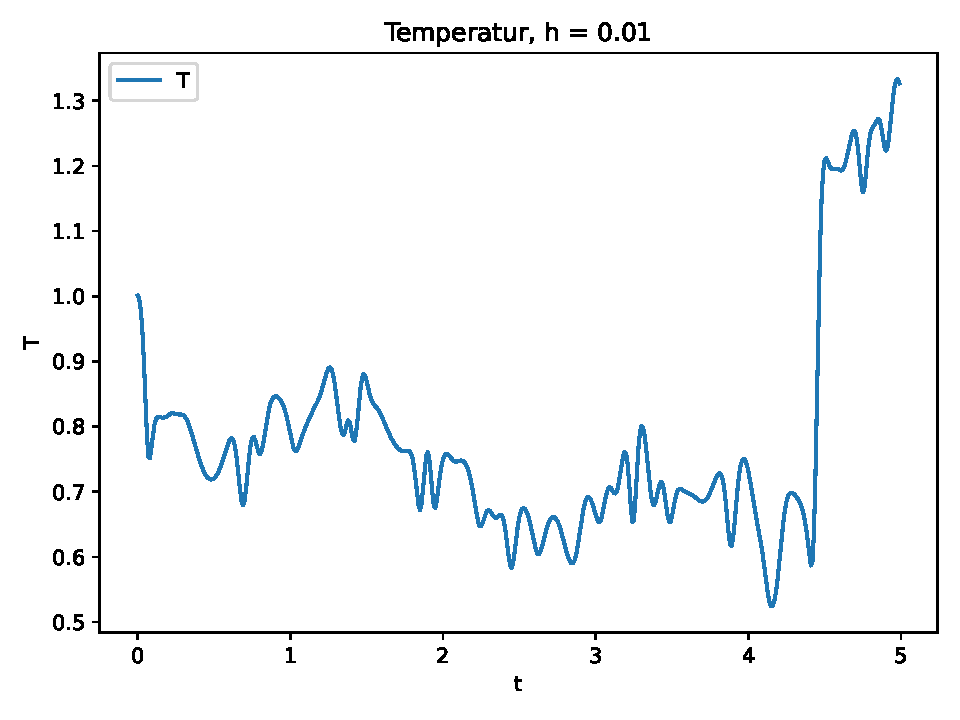
\includegraphics[width=\textwidth]{images/plot_T_16.pdf}
            \caption{The temperature of the 16 particle simulation over 5 seconds with a stepsize of 0.001.}
        \end{figure}        \begin{figure}
            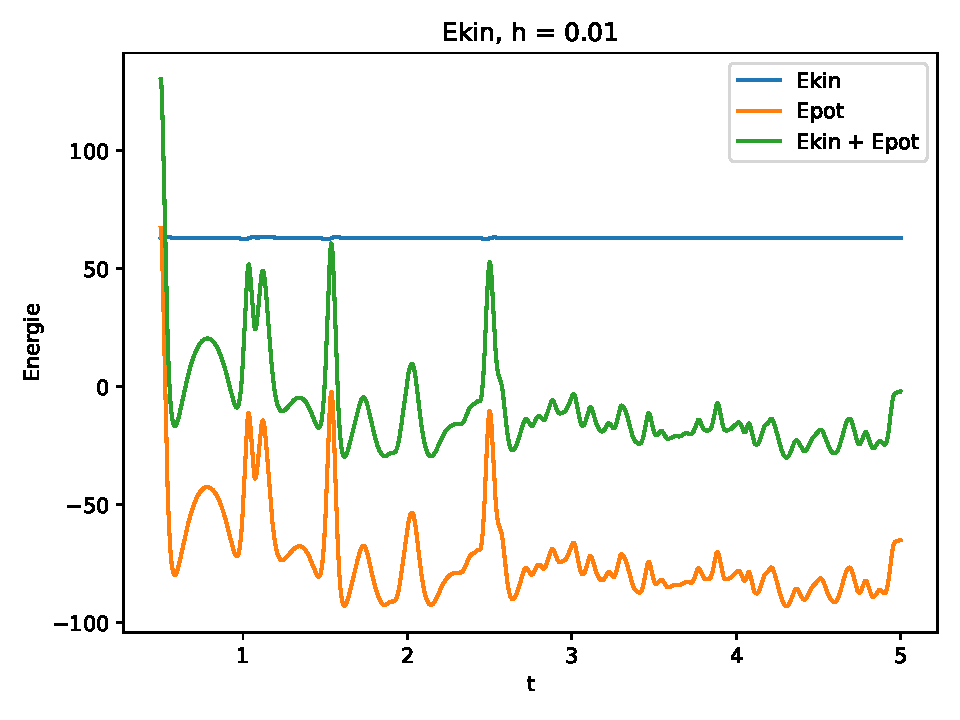
\includegraphics[width=\textwidth]{images/plot_E_64.pdf}
            \caption{The energy of the 64 particle simulation over 5 seconds with a stepsize of 0.001.}
        \end{figure}        \begin{figure}
            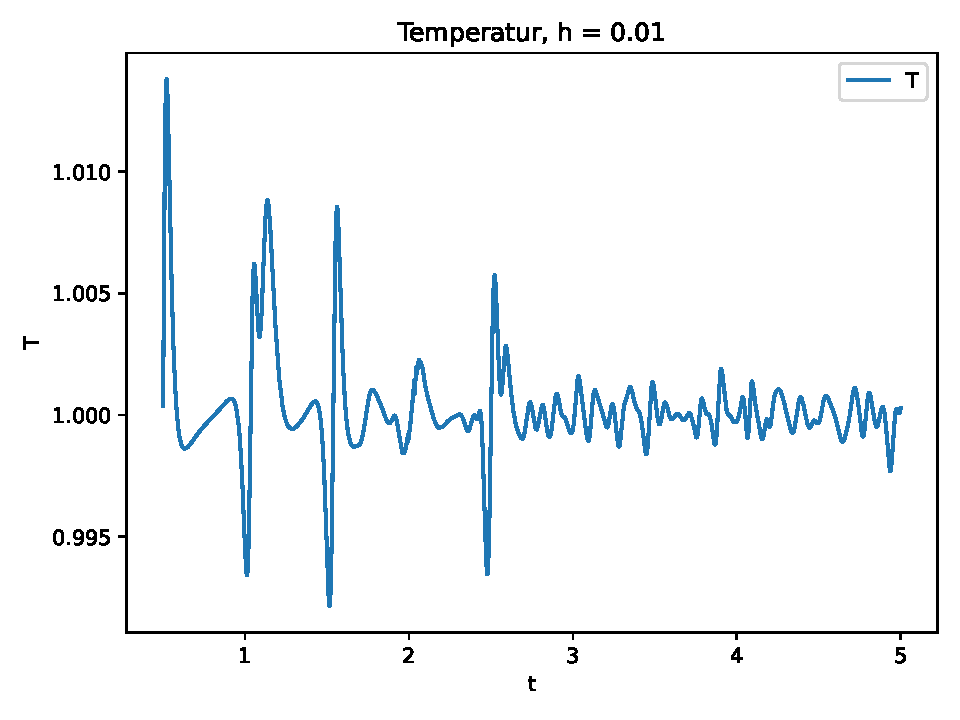
\includegraphics[width=\textwidth]{images/plot_T_64.pdf}
            \caption{The temperature of the 64 particle simulation over 5 seconds with a stepsize of 0.001.}
        \end{figure}        \begin{figure}
            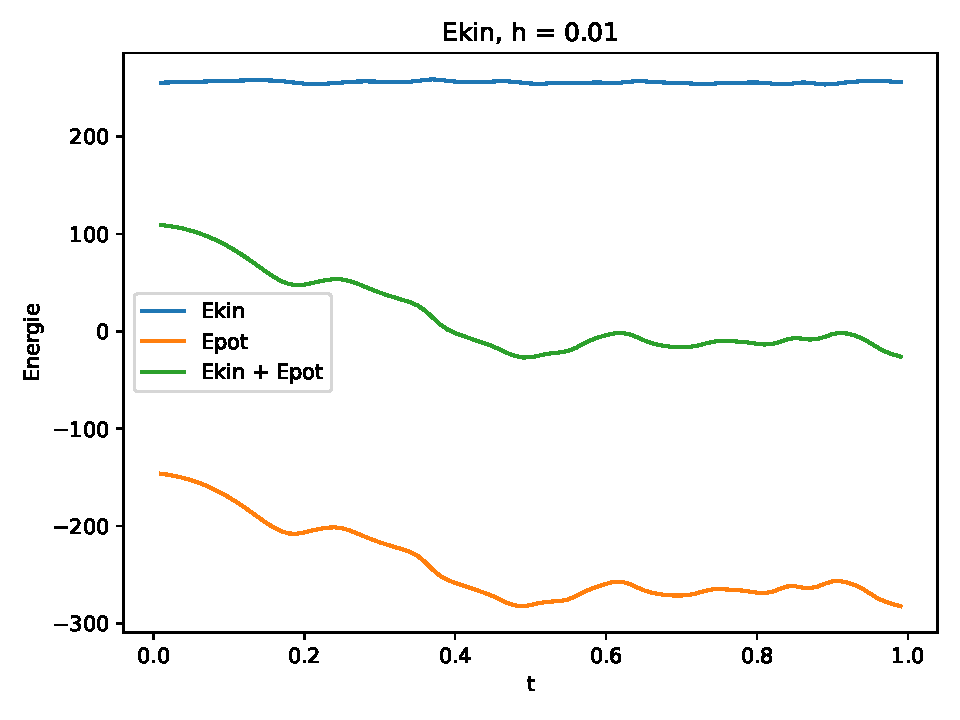
\includegraphics[width=\textwidth]{images/plot_E_256.pdf}
            \caption{The energy of the 256 particle simulation over 5 seconds with a stepsize of 0.001.}
        \end{figure}
        \begin{figure}
            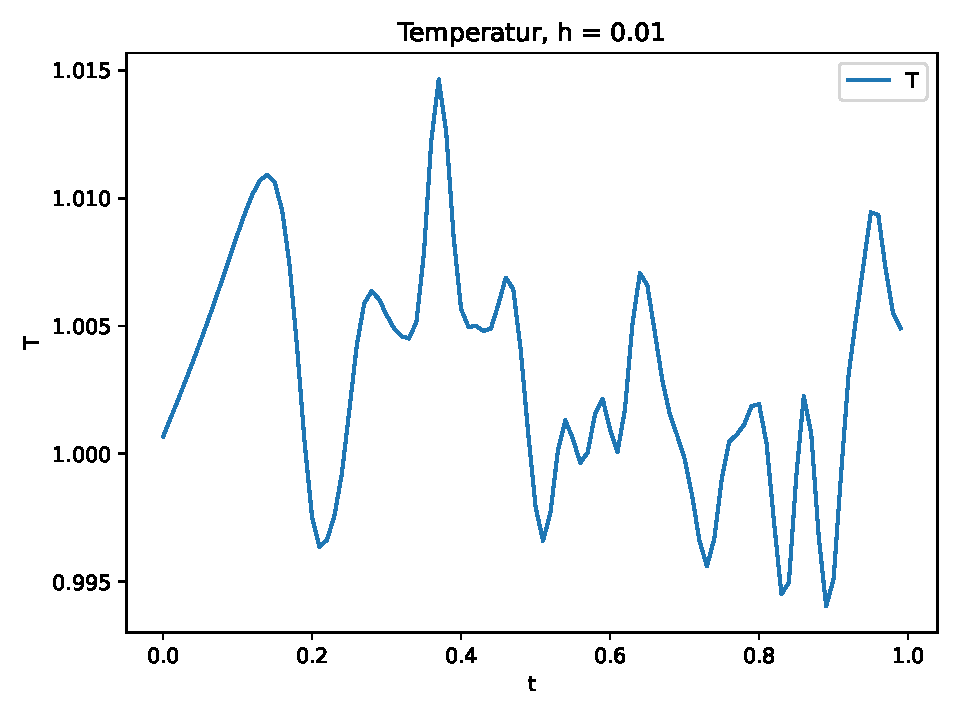
\includegraphics[width=\textwidth]{images/plot_T_256.pdf}
            \caption{The temperature of the 256 particle simulation over 5 seconds with a stepsize of 0.001.}
        \end{figure}
        \FloatBarrier
        Overall we expected a smaller fluctuation in both energy in temperature.
        We also expected the potential Energy to be equal to the kinectic energy.
        However the potential energy is about twice as big.
        The kinetic energy also does some really weird stuff if we dont rescale it with the thermostat after every step.
        This is probably not intended, but we dont really have the time to find the bug.
        With more time we probably could have fixed that mistake.
    \item[c)] It is 20 minutes before midnight right now and our code just started working kind of like it should so I am not sure if the simulation is going to produce results soon enough.
            Its five minutes before midnight and the programm is still running.
            So I guess this means we won't have plots on this part.
            Maybe I can append some plots after the due date.
    \item[d)]
        We implemented the isokinetic thermostat. 
        However, we did not really have the time to test it out properly.
        But what probably happens is a condensed matter phase.
        So the particles we build something like a grid or semi stable system.
    \item[e)]
    \begin{itemize}
        \item quantities that are kept constant are 
        \begin{itemize}
            \item particle number
            \item Volumen of the box 
            \item Basically the energy aswell
        \end{itemize}
        \item So the simulation is modelling a microcanonical esemble.
        \item No the isokinetic thermostat is not physically accurate. A more accuarte thermostat would be the Nose-Hoover Thermostat.
        This thermostat actually results in a boltzmann-distribution for the energy.
        \item First of all a chemical solution might be reactive. This could change the temperature over time.
        A chemical solution might also have particles of different mass. However this want change the esemble.
        Overall the most accuarte esemble would be the grand canonical esemble as the chemical potetntial stays the same, but the particle number changes.

    \end{itemize}
\end{itemize}
